%%%%%%%%%%%%%%%%%%%%%%%%%%%%%%% COMMENT THIS TO COMPILE main.tex %%%%%%%%%%%%%%%%%%%%%%%%%%%%%%%%
\documentclass[a4paper,12pt]{report}
\usepackage[english]{babel}
\usepackage[left=2cm,right=2cm,top=2cm,bottom=2cm]{geometry}
%\usepackage{mathtools}
\usepackage{amsthm}     % for definitions and theorems
\usepackage[many]{tcolorbox}    % boxes around definitions and theorems
%\usepackage{amsmath}
%\usepackage{nccmath}
\usepackage{amssymb}    % \ltimes
\usepackage{etoolbox}   % for start of Chapter
%\usepackage{amsfonts}
\usepackage{physics}    % for all Physics related
\usepackage{dsfont}     % for the identity matrix symbol \1
%\usepackage{mathrsfs}

\usepackage{titling}
\usepackage{indentfirst}

\usepackage{bm}
\usepackage[dvipsnames]{xcolor}
\usepackage{cancel}

\usepackage{xurl}
\usepackage[colorlinks=true]{hyperref}

\usepackage{float}
\usepackage{graphicx}
\usepackage{subcaption}
%\usepackage{tikz}

\usepackage{ctable}     % tabelas
\renewcommand{\P}{\phantom{+}}  % empty space to indent things
\usepackage{multirow}
\usepackage{tabulary}

%%%%%%%%%%%%%%%%%%%%%%%%%%%%%%%%%%%%%%%%%%%%%%%%%%%

\newcommand{\eps}{\epsilon}
\newcommand{\vphi}{\varphi}
\newcommand{\cte}{\text{cte}}

\newcommand{\N}{{\mathbb{N}}}
\newcommand{\Z}{{\mathbb{Z}}}
%\newcommand{\Q}{{\mathbb{Q}}}
\newcommand{\C}{{\mathbb{C}}}
\renewcommand{\S}{{\hat{S}}}
%\renewcommand{\H}{\s{H}}

\renewcommand{\a}{{\vb{a}}}
\renewcommand{\b}{{\vb{b}}}
\renewcommand{\d}{{\dagger}}
\newcommand{\up}{{\uparrow}}
\newcommand{\down}{{\downarrow}}
\newcommand{\hc}{{\text{h.c.}}}

\newcommand{\ihat}{\bm{\hat{\imath}}}
\newcommand{\jhat}{\bm{\hat{\jmath}}}
\newcommand{\khat}{\bm{\hat{k}}}

\newcommand{\0}{{\vb{0}}}
\newcommand{\1}{\mathds{1}}
\newcommand{\E}{{\vb{E}}}
\newcommand{\B}{{\vb{B}}}
\renewcommand{\u}{{\vb{u}}}
\renewcommand{\v}{{\vb{v}}}
\renewcommand{\r}{{\vb{r}}}
\newcommand{\R}{{\vb{R}}}
\newcommand{\Q}{{\vb{Q}}}
\newcommand{\G}{{\vb{G}}}
\newcommand{\g}{{\vb{g}}}
\renewcommand{\k}{{\vb{k}}}
\newcommand{\K}{{\vb{K}}}
\newcommand{\p}{{\vb{p}}}
\newcommand{\q}{{\vb{q}}}
\newcommand{\F}{{\vb{F}}}
\renewcommand{\t}{{\vb{t}}}
\newcommand{\vtau}{{\bm{\tau}}}
\newcommand{\vdelta}{{\bm{\delta}}}

% COLORED SYMMETRY ELEMENTS
\newcommand{\Ct}{{\textcolor{Cyan}{C_3}}}
\newcommand{\Ctn}[1]{{\textcolor{Cyan}{C_3^{\textcolor{black}{#1}}}}}
\newcommand{\Cs}{{\textcolor{ForestGreen}{C_6}}}
\newcommand{\Csn}[1]{{\textcolor{ForestGreen}{C_6^{\textcolor{black}{#1}}}}}
\newcommand{\sd}{{\textcolor{RoyalBlue}{\sigma_d}}}
\newcommand{\sdn}[1]{{\textcolor{RoyalBlue}{\sigma_d^{\textcolor{black}{#1}}}}}
\newcommand{\sdp}{{\textcolor{RoyalBlue}{\sigma_d'}}}
\newcommand{\sdpp}{{\textcolor{RoyalBlue}{\sigma_d''}}}
\newcommand{\sv}{{\textcolor{Orange}{\sigma_v}}}
\newcommand{\svn}[1]{{\textcolor{Orange}{\sigma_v^{\textcolor{black}{#1}}}}}
\newcommand{\svp}{{\textcolor{Orange}{\sigma_v'}}}
\newcommand{\svpp}{{\textcolor{Orange}{\sigma_v''}}}

\newcommand{\s}{\sigma}
%\newcommand{\prodint}[2]{\left\langle #1 , #2 \right\rangle}
\newcommand{\cc}[1]{\overline{#1}}
\newcommand{\Eval}[3]{\eval{\left( #1 \right)}_{#2}^{#3}}
\newcommand{\sg}[2]{\{ #1 \mid #2 \}}

\newcommand{\unit}[1]{\; \mathrm{#1}}

\newcommand{\n}{\medskip}
\newcommand{\e}{\quad \mathrm{and} \quad}
\newcommand{\ou}{\quad \mathrm{or} \quad}
\newcommand{\virg}{\, , \;}
\newcommand{\ptodo}{\forall \,}
\renewcommand{\implies}{\; \Rightarrow \;}
%\newcommand{\eqname}[1]{\tag*{#1}} % Tag equation with name

\setlength{\droptitle}{-7em}

\makeatletter
\patchcmd{\chapter}{\if@openright\cleardoublepage\else\clearpage\fi}{}{}{}  % start 'Chapter' at the same page. needs package etoolbox
\makeatother

%% Theorems, definitions, proofs
\theoremstyle{definition}

\newtheorem{definition}{Definition}[section]
\tcolorboxenvironment{definition}{
  colback=blue!5!white,
  boxrule=0pt,
  boxsep=1pt,
  left=2pt,right=2pt,top=2pt,bottom=2pt,
  oversize=2pt,
  sharp corners,
  before skip=\topsep,
  after skip=\topsep,
}

\newtheorem{theorem}{Theorem}[section]
\tcolorboxenvironment{theorem}{
  colback=blue!5!white,
  boxrule=0pt,
  boxsep=1pt,
  left=2pt,right=2pt,top=2pt,bottom=2pt,
  oversize=2pt,
  sharp corners,
  before skip=\topsep,
  after skip=\topsep,
}

\begin{document}
%%%%%%%%%%%%%%%%%%%%%%%%%%%%%%% COMMENT THIS TO COMPILE main.tex %%%%%%%%%%%%%%%%%%%%%%%%%%%%%%%%


%%%%%%%%%%%%%%%%%%%%%%%%%%%%%%%%%%%%%%%%%%%%%%%%%%%%%%%%%%%%%%%%%%%%%%%%%%%%%%%%%%%%%%%%%%%%%%%%%%
\chapter{Topological heavy fermion} \label{ch:topoheavyfermion}
%%%%%%%%%%%%%%%%%%%%%%%%%%%%%%%%%%%%%%%%%%%%%%%%%%%%%%%%%%%%%%%%%%%%%%%%%%%%%%%%%%%%%%%%%%%%%%%%%%

\textbf{PLAGIADO DO TOPOHEAVYFERMION}

In the current manuscript, nevertheless, we find it possible to write down a fully symmetric model that has a simple real space picture, which, remarkably and elegantly, solves the aforementioned puzzles.
We reformulate and map the interacting MATBG as an effective topological heavy fermion system, which consists of local orbitals (\(f\)) centered at the AA-stacking regions and delocalized topological conduction bands (\(c\)). The \(f\)-electrons are so localized that they have an almost zero kinetic energy (\(\sim 0.1 \, \text{meV}\)) but a strong on-site Coulomb repulsion that we compute to be \(\sim 60 \, \text{meV}\). The \(c\)-electrons carry the symmetry anomaly and have unbounded kinetic energies. The actual flat bands of the BM model are from a hybridization (\(\sim 20 \, \text{meV}\)) between the \(f\)- and \(c\)-bands. The interacting Hamiltonian also couples the \(f\) and \(c\) electrons through the presence of several types of interactions.
Using this model, the ground states \cite{1, 2, 44, 50, 53, 65, 68, 71, 77, 84–86, 114} and their topologies can be understood in a simple, physical picture. The quasi-particle excitation bandwidth can even be analytically determined.

\textbf{PLAGIADO DO TOPOHEAVYFERMION}

\begin{figure}[H]
\centering
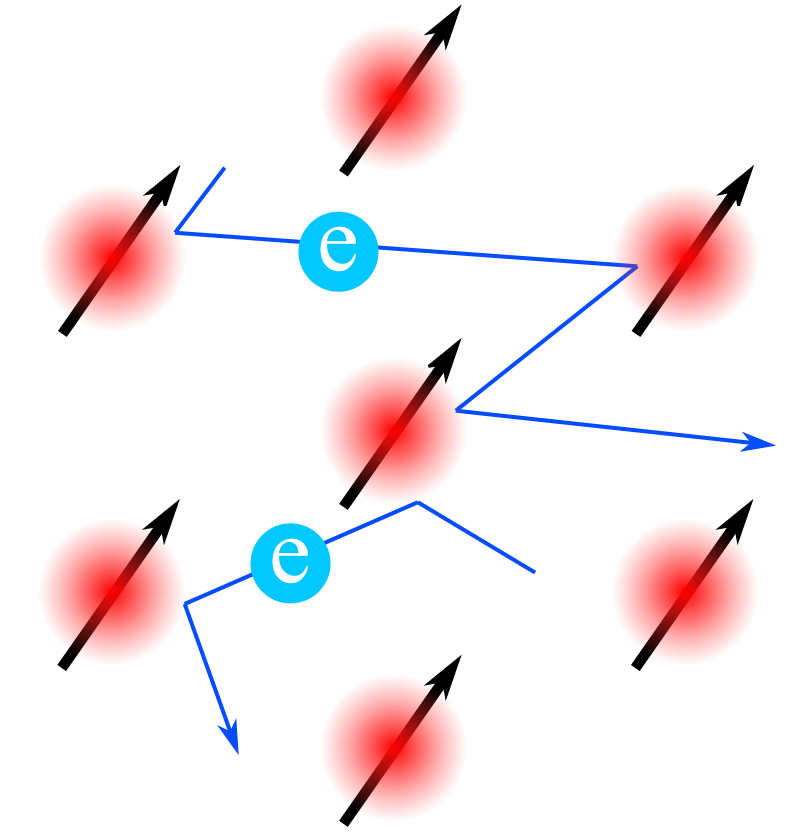
\includegraphics[width=0.3\linewidth]{fig/topoheavyfermion_fc_electrons.png}
\caption{\textbf{Plagiado:} A sketch of the moiré unit cell of MATBG and its heavy fermion analog, where the local moments and itinerant electrons are formed by the effective $f$-orbitals at the AA-stacking regions and topological conduction bands}
\label{fig:topoheavyfermion_fc_electrons}
\end{figure}

\textbf{MAKE A FIGURE OF BM BANDS WITH THEIR REPRESENTATIONS LABELED, WITH $\Gamma_3$.}

\n

\textbf{PLAGIADO DO TOPOHEAVYFERMION}

Here we resolve the fragile topology by involving higher energy bands. Suppose we can “borrow” a \(\Gamma_3\) irrep from higher (\(\sim 20 \, \text{meV}\)) energy bands and use it to replace the \(\Gamma_1 \oplus \Gamma_2\) states; then the replaced irreps - \(\Gamma_3, M_1 \oplus M_2, K_2K_3\) - are consistent with \(p_x \pm i p_y\) orbitals located at the triangular lattice. We hence introduce two trial Gaussian-type Wannier functions (WFs) that transform as \(p_x \pm i p_y\) orbitals under the crystalline symmetries.
As indicated by the overlaps between the trial WFs and the Bloch bands (Fig. 1(a)), the trial WFs are supported by the flat band states at \(k\) away from \(\Gamma M\) and by the lowest higher energy band states around \(\Gamma M\). Feeding the overlaps into the program Wannier90 \cite{121–123}, we obtain the corresponding maximally localized WFs, density profile of which is shown in Fig. 1(b) \cite{115}. (Similar local states are also discussed using different methods in Refs. \cite{38, 112}.)
These WFs are extremely localized - their nearest neighbor hoppings are about \(0.1 \, \text{meV}\) - and span 96\% of the flat bands.

\textbf{PLAGIADO DO TOPOHEAVYFERMION}

\n

\textbf{PLAGIADO DO TOPOHEAVYFERMION}

To recover the irreps and topology of the middle two bands, we have to take into account the remaining 4\% states, without which the localized electrons could not form a superconductor. To do this, we define the projector into the WFs as \( P \), the projector into the lowest six bands (per spin valley) as \( I \), and divide the low-energy BM Hamiltonian \( H_{\text{BM}} \) into four parts: \( H(f) = P H_{\text{BM}} P \), \( H(c) = Q H_{\text{BM}} Q \), \( H(fc) = P H_{\text{BM}} Q \), \( H(cf) = H(fc)^\dagger \), where \( Q = I - P \), \( H(c) \) is the remaining Hamiltonian, and \( H(fc) + \text{h.c.} \) is the coupling between WFs and the remaining states. As the couplings between WFs are extremely weak (\(\sim 0.1\, \text{meV}\)), we find \( H(f) \approx 0 \). Since the two states in \( P \) form \(\Gamma_3\) at \(\Gamma_M\), the four states in \( Q \) must form \(\Gamma_3 \oplus \Gamma_1 \oplus \Gamma_2\) at \(\Gamma_M\) due to the irrep counting.

Due to the crystalline and \( P \) symmetries, \( H(c) \) in the valley \( \eta \) takes the form
\[
H(c,\eta)(k) =
\begin{pmatrix}
0_{2 \times 2} & v^\ast (\eta k_x \sigma_0 + i k_y \sigma_z) \\
v^\ast (\eta k_x \sigma_0 - i k_y \sigma_z) & M \sigma_x
\end{pmatrix}
\]
to linear order of \( k \), where the first \( 2 \times 2 \) block is spanned by the \(\Gamma_3\) states and the second \( 2 \times 2 \) block is spanned by the \(\Gamma_1 \oplus \Gamma_2\) states. The \(\Gamma_1\) and \(\Gamma_2\) states are split by the \( M \) term (blue bands in Fig. 1(c)), while the \(\Gamma_3\) states form a quadratic touching at \( k = 0 \), which is shown in Ref. \cite{115} to be responsible for the symmetry anomaly \cite{104} jointly protected by \( C_{2z}T \) and \( P \).

The coupling \( H(fc) \) in the valley \( \eta \) has the form
\[
H(fc,\eta)(k) =
\begin{pmatrix}
\gamma \sigma_0 + v'^\ast (\eta k_x \sigma_x + k_y \sigma_y), & 0_{2 \times 2}
\end{pmatrix}
\]
where the second block is computed to be extremely small and hence is omitted and written as \( 0_{2 \times 2} \). \( H(fc,\eta) \) will gap \( H(c,\eta) \), and hence provides both the single-particle gap and the flat-band topology of the BM model. Using a set of commonly adopted parameters for MATBG, we find \( v^\ast = -4.303\, \text{eV} \cdot \text{Å} \), \( M = 3.697\, \text{meV} \), \( \gamma = -24.75\, \text{meV} \), and \( v'^\ast = 1.622\, \text{eV} \cdot \text{Å} \).

Since the WFs and the remaining "c" degrees of freedom have localized and plane-wave-like wave functions, respectively, we make the analogy with local orbitals and conduction bands in heavy fermion systems. We refer to them as local \( f \)-orbitals and (topological) conduction \( c \)-bands, respectively. We use \( f_{R\alpha\eta s} \) (\(\alpha = 1, 2, \eta = \pm, s = \uparrow, \downarrow\)) to represent the annihilation operator of the \(\alpha\)-th WF of the valley \( \eta \) and spin \( s \) at the moiré unit cell \( R \). We use \( c_{ka\eta s} \) (\( a = 1, 2, 3, 4 \)) to represent the annihilation operator of the \( a\)-th conduction band basis of the valley \( \eta \) and spin \( s \) at the moiré momentum \( k \). The single-particle Hamiltonian can be written as
\[
\hat{H}_0 =
\sum_{|k| < \Lambda_c}
\sum_{aa'\eta s}
H(c,\eta)_{aa'}(k) c^\dagger_{ka\eta s} c_{ka'\eta s}
+ \frac{1}{\sqrt{N}}
\sum_{|k| < \Lambda_c}
\sum_{R}
\sum_{\alpha a \eta s}
\left( e^{i k \cdot R - \frac{|k|^2 \lambda^2}{2}}
H(fc,\eta)_{\alpha a}(k) f^\dagger_{R\alpha\eta s} c_{ka\eta s} + \text{h.c.} \right),
\]
where \( \Lambda_c \) is the momentum cutoff for the \( c \)-electrons, \( a_M \) is the moiré lattice constant, \( N \) is the number of moiré unit cells in the system, and \( \lambda \), which is found to be \( 0.3375 a_M \), is a damping factor proportional to the size of WFs. We plot the band structure of \( \hat{H}_0 \) in Fig. 1(c), where the splitting of the two \(\Gamma_3\) states is given by \( 2|\gamma| \) and the bandwidth of the two flat bands is given by \( 2M \approx 7.4\, \text{meV} \). The spectrum of \( \hat{H}_0 \) matches very well with the BM model (Fig. 1(a)) in the energy range \([-70\, \text{meV}, 70\, \text{meV}]\).

\textbf{PLAGIADO DO TOPOHEAVYFERMION}

\n\n


To resolve this Wannier obstruction, we incorporate the nearest higher-energy bands, which are characterized by the \(\Gamma_3\) irrep at the \(\Gamma_M\) point \cite{topoheavyfermion2022}. These higher-energy bands hybridize with the two middle bands, allowing us to isolate the trivial bands. These trivial bands form the band representation:
\begin{equation} \label{eq:trivial-irreps}
G_E^{1a}(2) = [E]_{1a} \uparrow G: \quad \Gamma_3(2); \; M_1(1) \oplus M_2(1); \; K_2 K_3(2),
\end{equation}
where \([E]_{1a}\) corresponds to \(p_x \pm i p_y\)-like orbitals at the \(1a\) Wyckoff position.

We ``borrow'' a $\Gamma_3$ irrep from these higher-energy bands to replace the $\Gamma_1 \oplus \Gamma_2$ states. The resulting irreps $\Gamma_3$, $M_1 \oplus M_2$, $K_2 K_3$ are consistent with $p_x \pm i p_y$ orbitals on a triangular lattice. To model this, Gaussian Wannier functions (WFs) that transform as $p_x \pm i p_y$ under the crystal symmetries are introduced.

Using the maximal localization procedure \cite{maxlocalWFs_marzari2012, wannier90}, we find that these WFs are highly localized, supported by flat band states away from $\Gamma_M$, and by low-energy states near $\Gamma_M$. However, to fully account for the superconducting properties, it is crucial to include the remaining states. To achieve this, we define projectors $\bP$ (onto the WFs) and $\I$ (onto the lowest six bands per spin-valley), and decompose the BM Hamiltonian $H_\text{BM}$ into the following components:
\begin{equation} \label{eq:projected_hamiltonians_WFs_PQ}
H^{(f)} = \bP H_\text{BM} \bP, \quad H^{(c)} = \bQ H_\text{BM} \bQ, \quad H^{(fc)} = \bP H_\text{BM} \bQ, \quad H^{(cf)} = H^{(fc)\dagger},
\end{equation}
where $\bQ = \I - \bP$. Since the coupling between WFs is extremely weak, the approximation $H^{(f)} \approx 0$ proves to be highly accurate.

The two states in $\bP$ form $\Gamma_3$ at $\Gamma_M$, while the four states in $\bQ$ form $\Gamma_3 \oplus \Gamma_1 \oplus \Gamma_2$. The remaining Hamiltonian $H^{(c)}$ in valley $\eta$ is expressed as:
\begin{equation} \label{eq:H(c)_topoheavyfermion}
H^{(c, \eta)}(\k) =
\begin{pmatrix}
0_{2\times 2} & v_* (\eta k_x \sigma_0 + i k_y \sigma_z) \\
v_* (\eta k_x \sigma_0 - i k_y \sigma_z) & M \sigma_x
\end{pmatrix}.
\end{equation}

The coupling $H^{(fc)}$ takes the form:
\begin{equation} \label{eq:H(fc)_topoheavyfermion}
H^{(fc, \eta)}(\k) =
\begin{pmatrix}
\gamma \sigma_0 + v'_* (\eta k_x \sigma_x + k_y \sigma_y) & 0_{2\times 2}
\end{pmatrix},
\end{equation}
which introduces a gap in $H^{(c, \eta)}$, establishing the flat band topology of the BM model.

Using standard parameters for MATBG, this mapping provides the parameter values:
\begin{equation} \label{eq:paramaters_topoheavyfermion}
v^\star = -4.303 \, \text{eV} \cdot \AA, \quad M = 3.697 \, \text{meV}, \quad \gamma = -24.75 \, \text{meV}, \quad v'^\star = 1.622 \, \text{eV} \cdot \AA.
\end{equation}

By diagonalizing the resulting 6-band model for the valley $\eta = +$, constructed from the Hamiltonians $H^{(c,\eta)}$ and $H^{(fc,\eta)}$, we obtain the results shown in Figure \ref{fig:thf-exploration}. We analyze the cases where certain parameters are set to zero to study the model's behavior.

\begin{figure}[H]
\centering
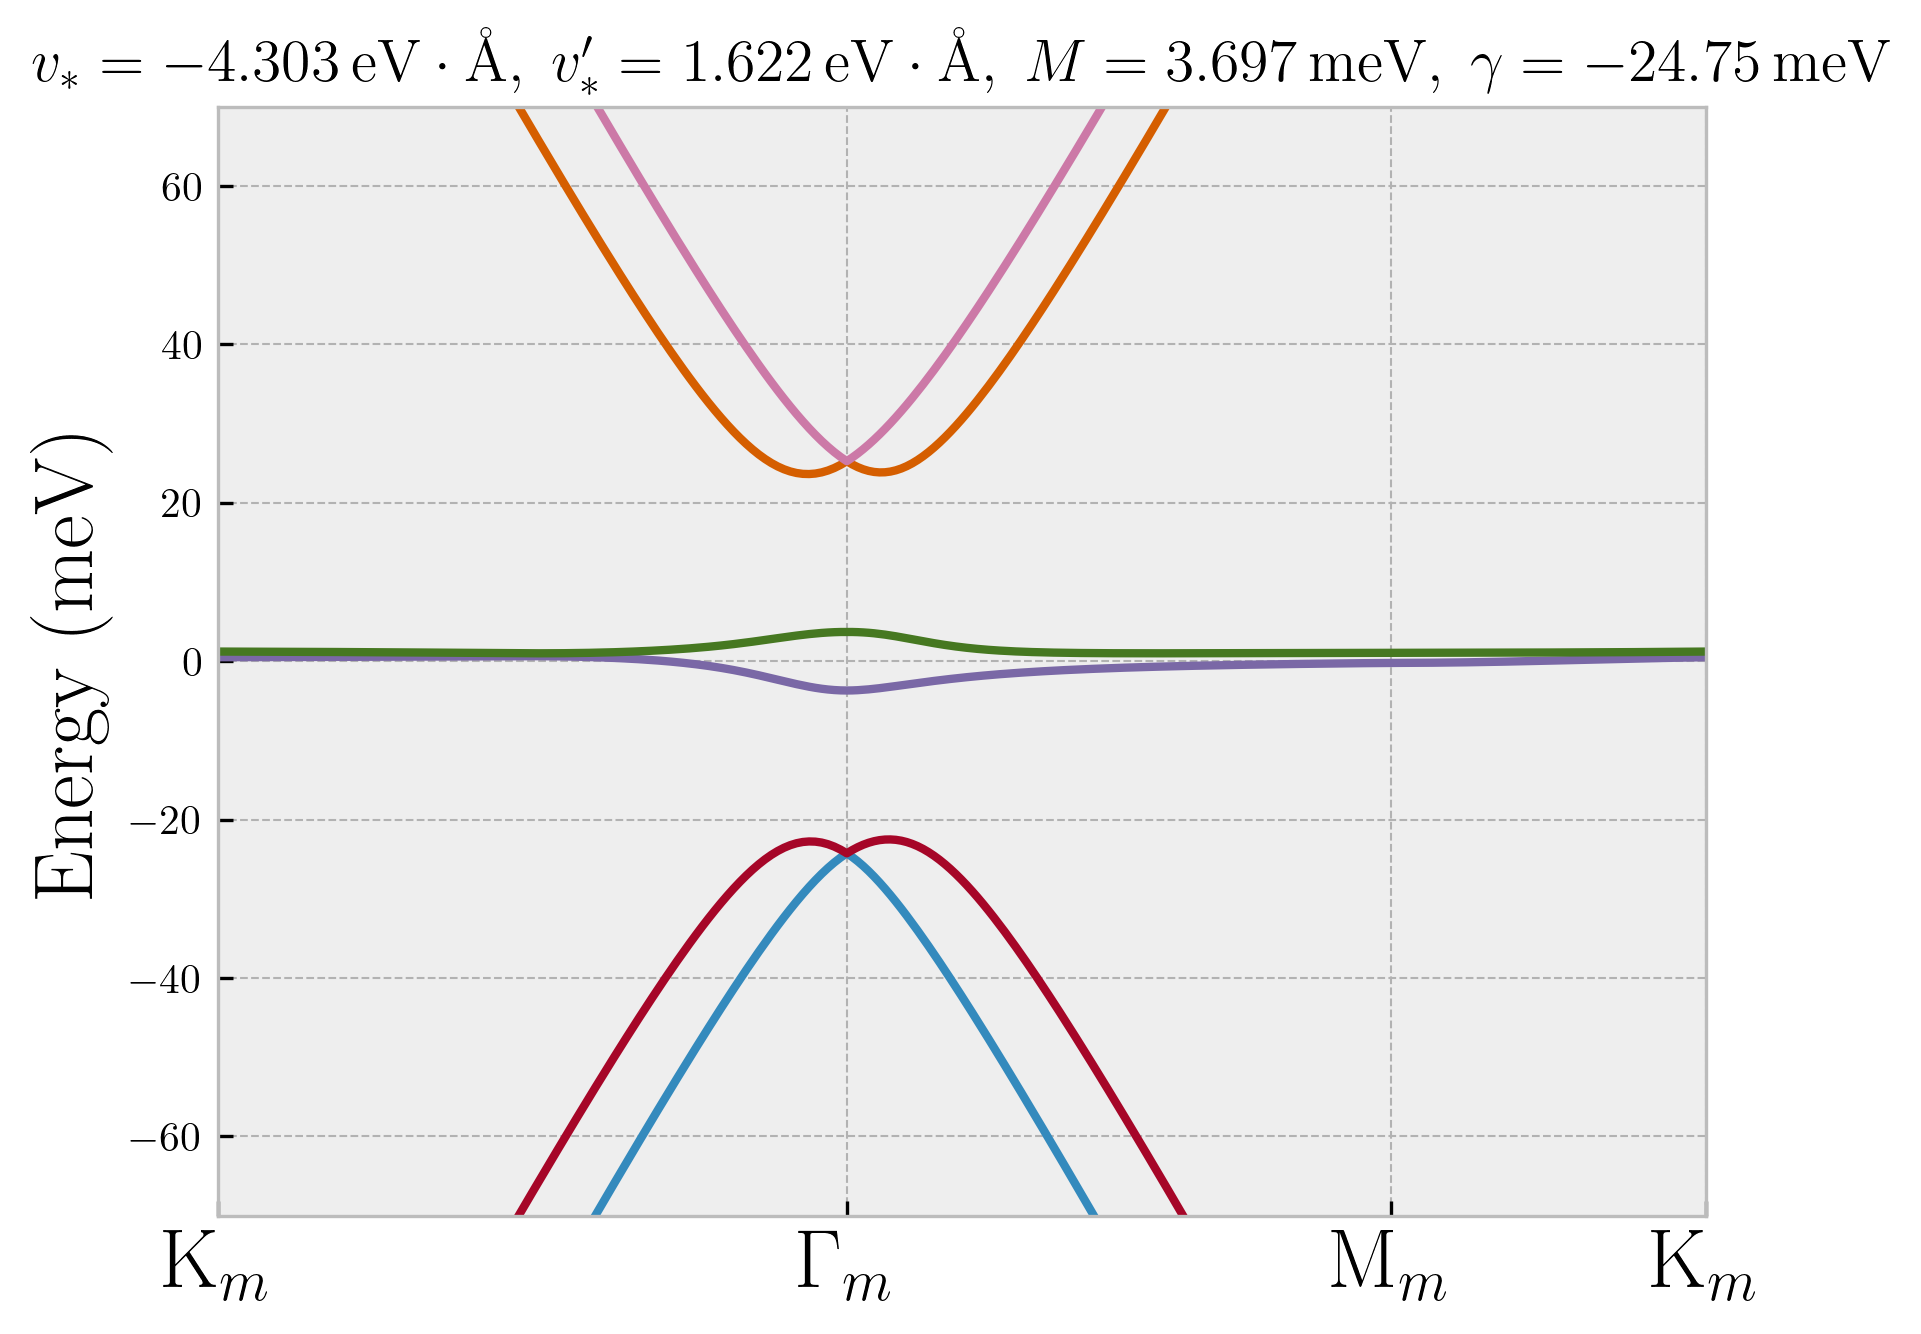
\includegraphics[height=0.35\linewidth]{fig/thf-correct_params.png} \hfill
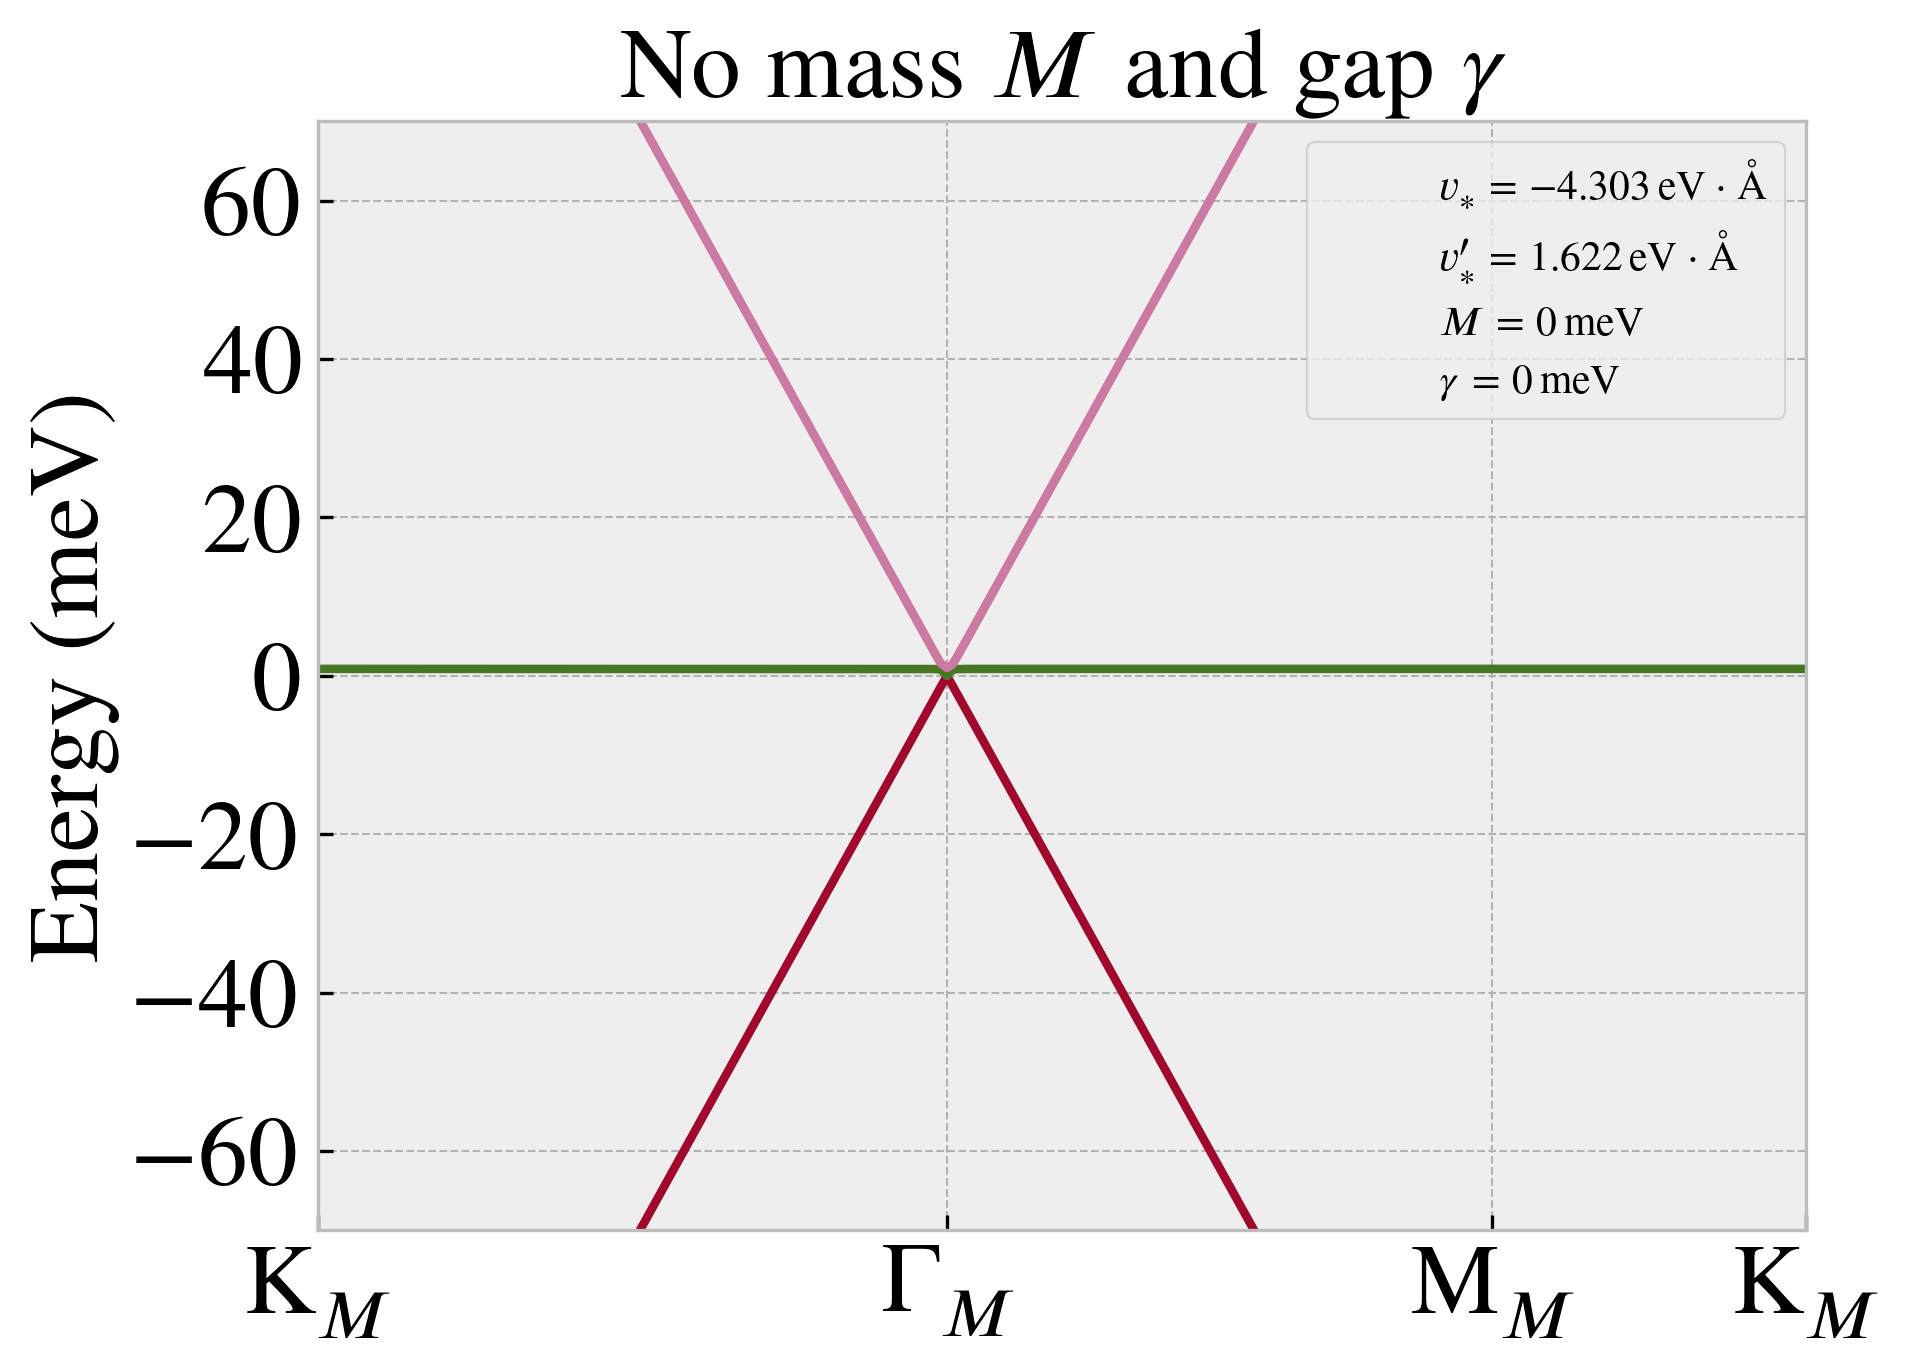
\includegraphics[height=0.35\linewidth]{fig/thf-no_M_no_gamma.png}
%%%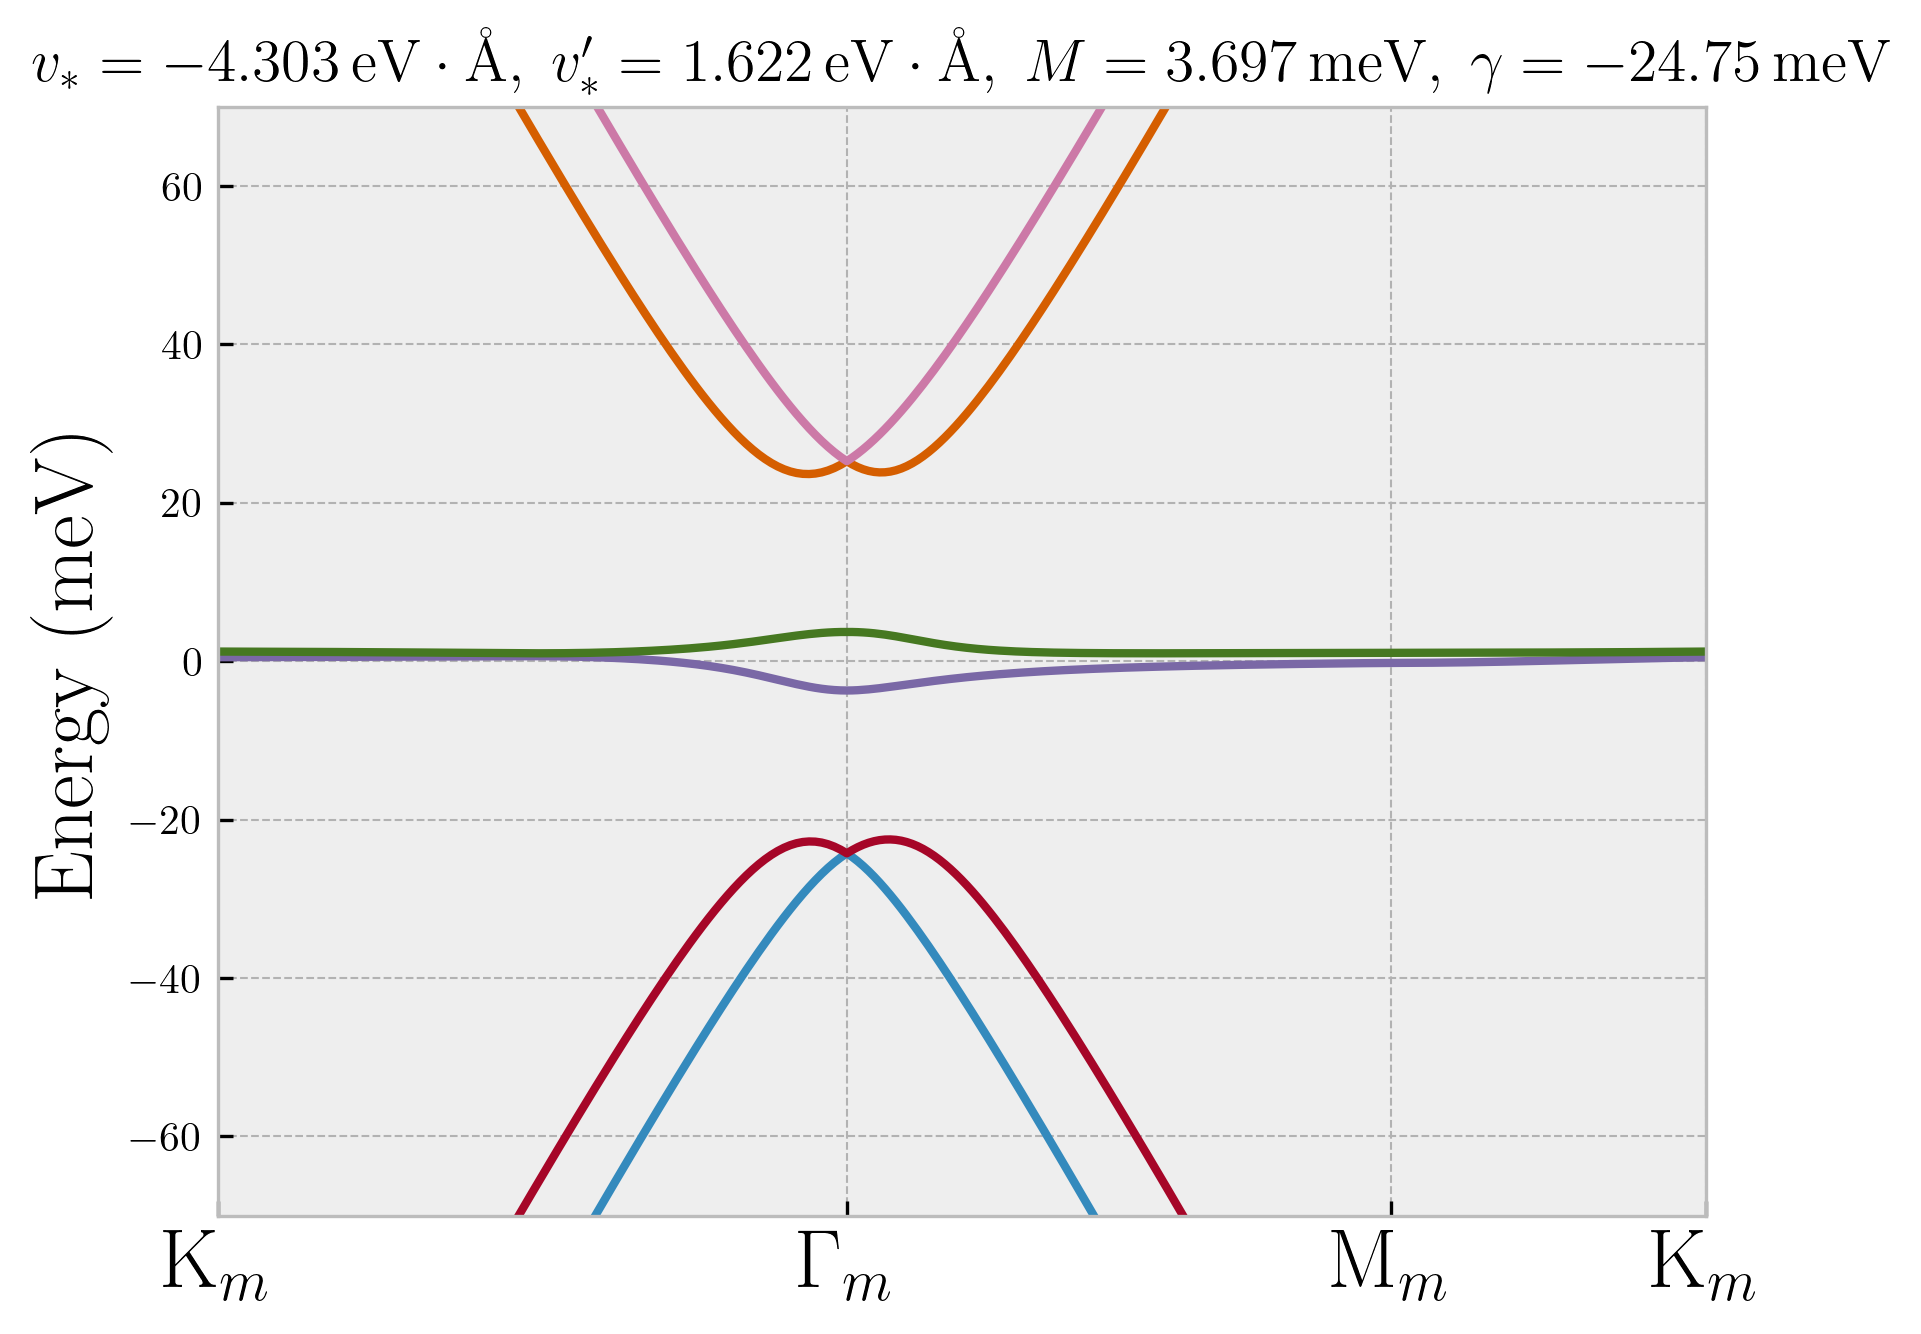
\includegraphics[height=0.35\linewidth]{fig/thf-correct_params.png}
%%%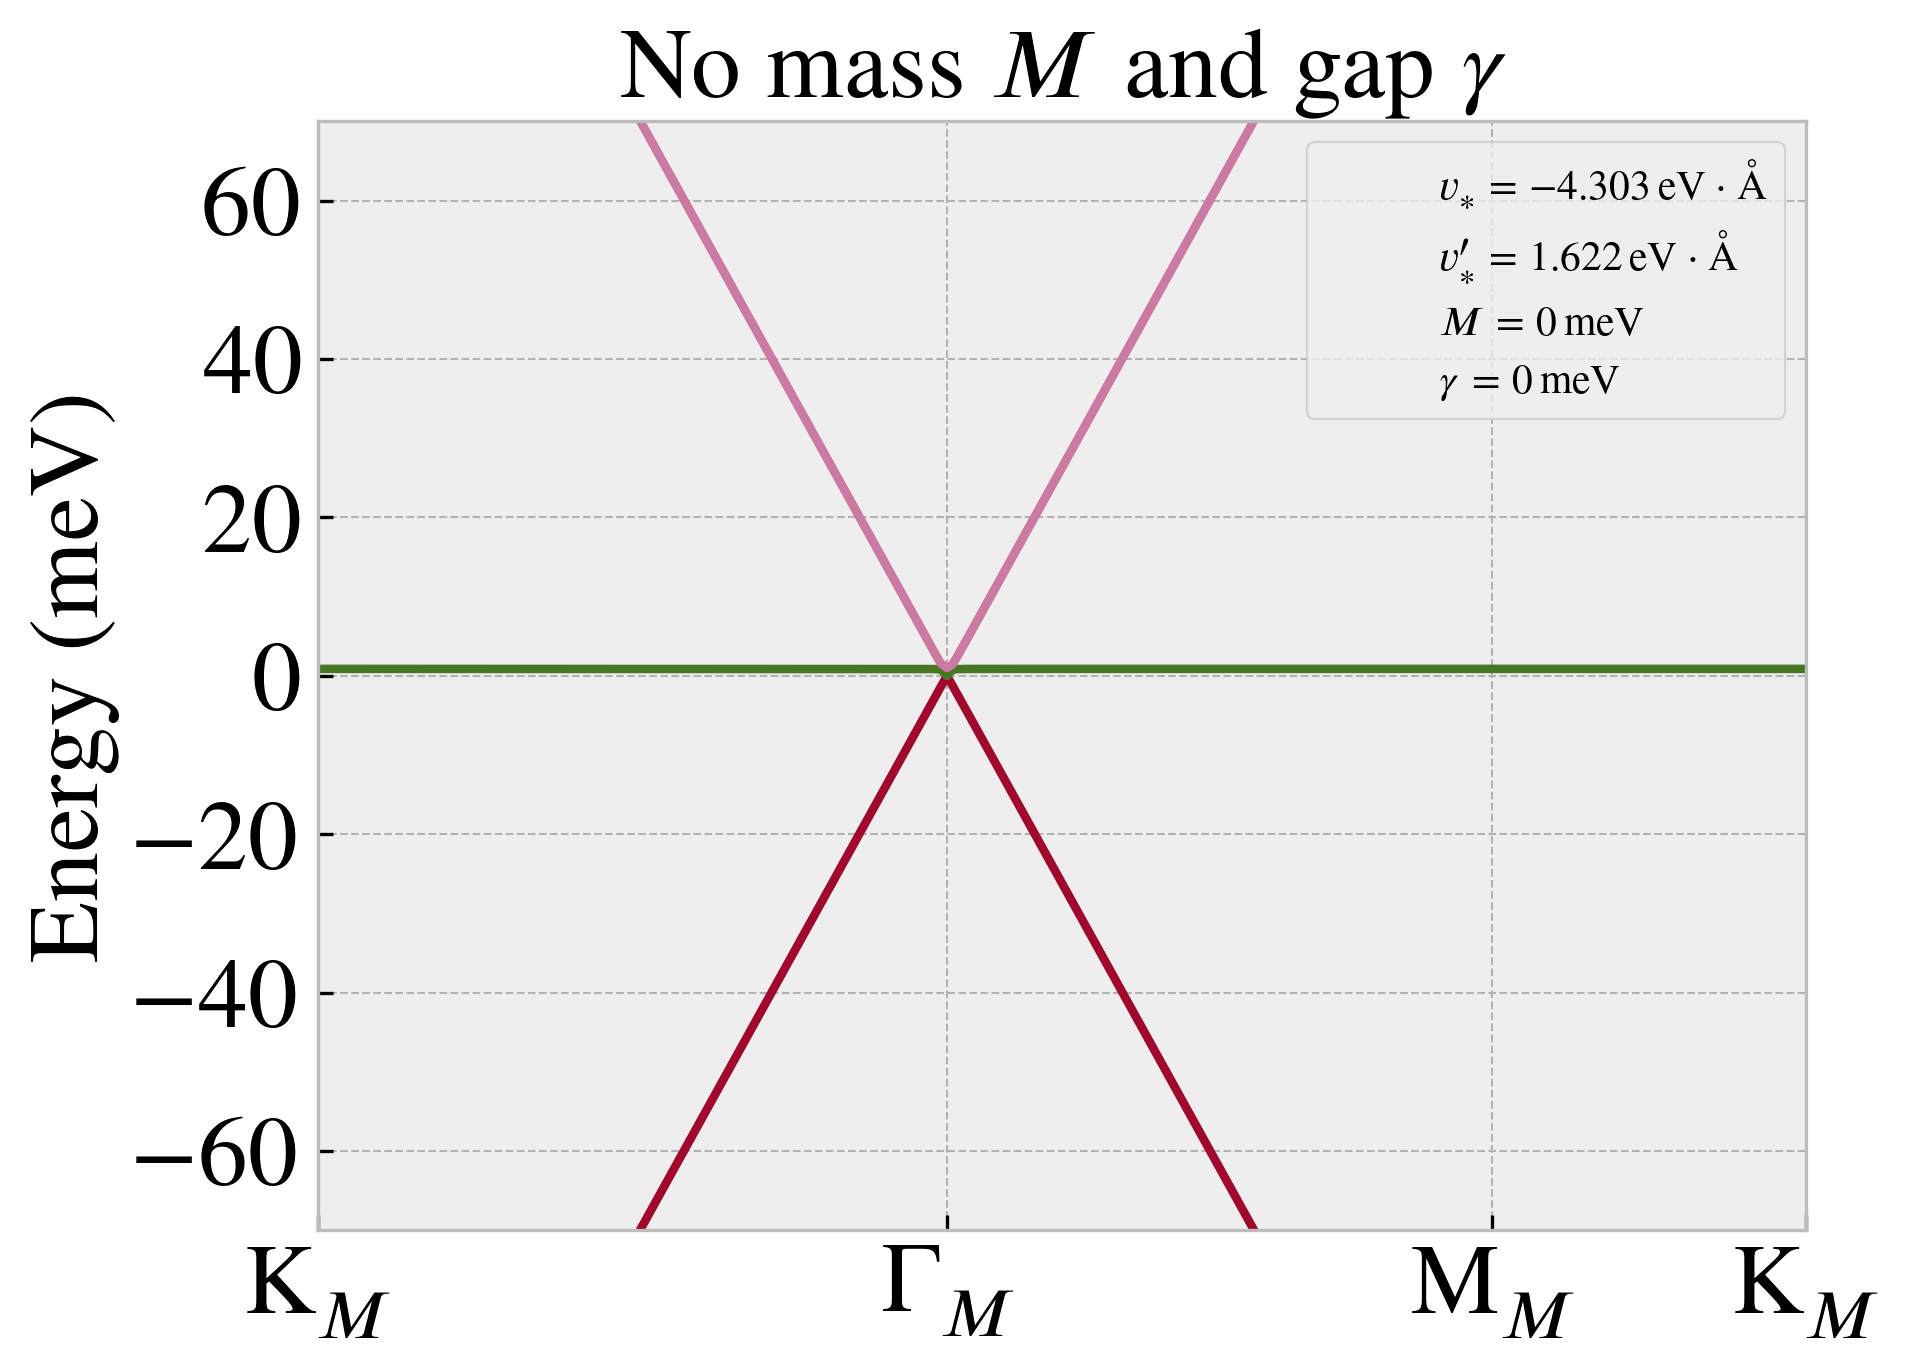
\includegraphics[height=0.35\linewidth]{fig/thf-no_M_no_gamma.png}
%%\caption{}
%\label{fig:thf-correct_params}
%\end{figure}
%\begin{figure}[H]
%\centering
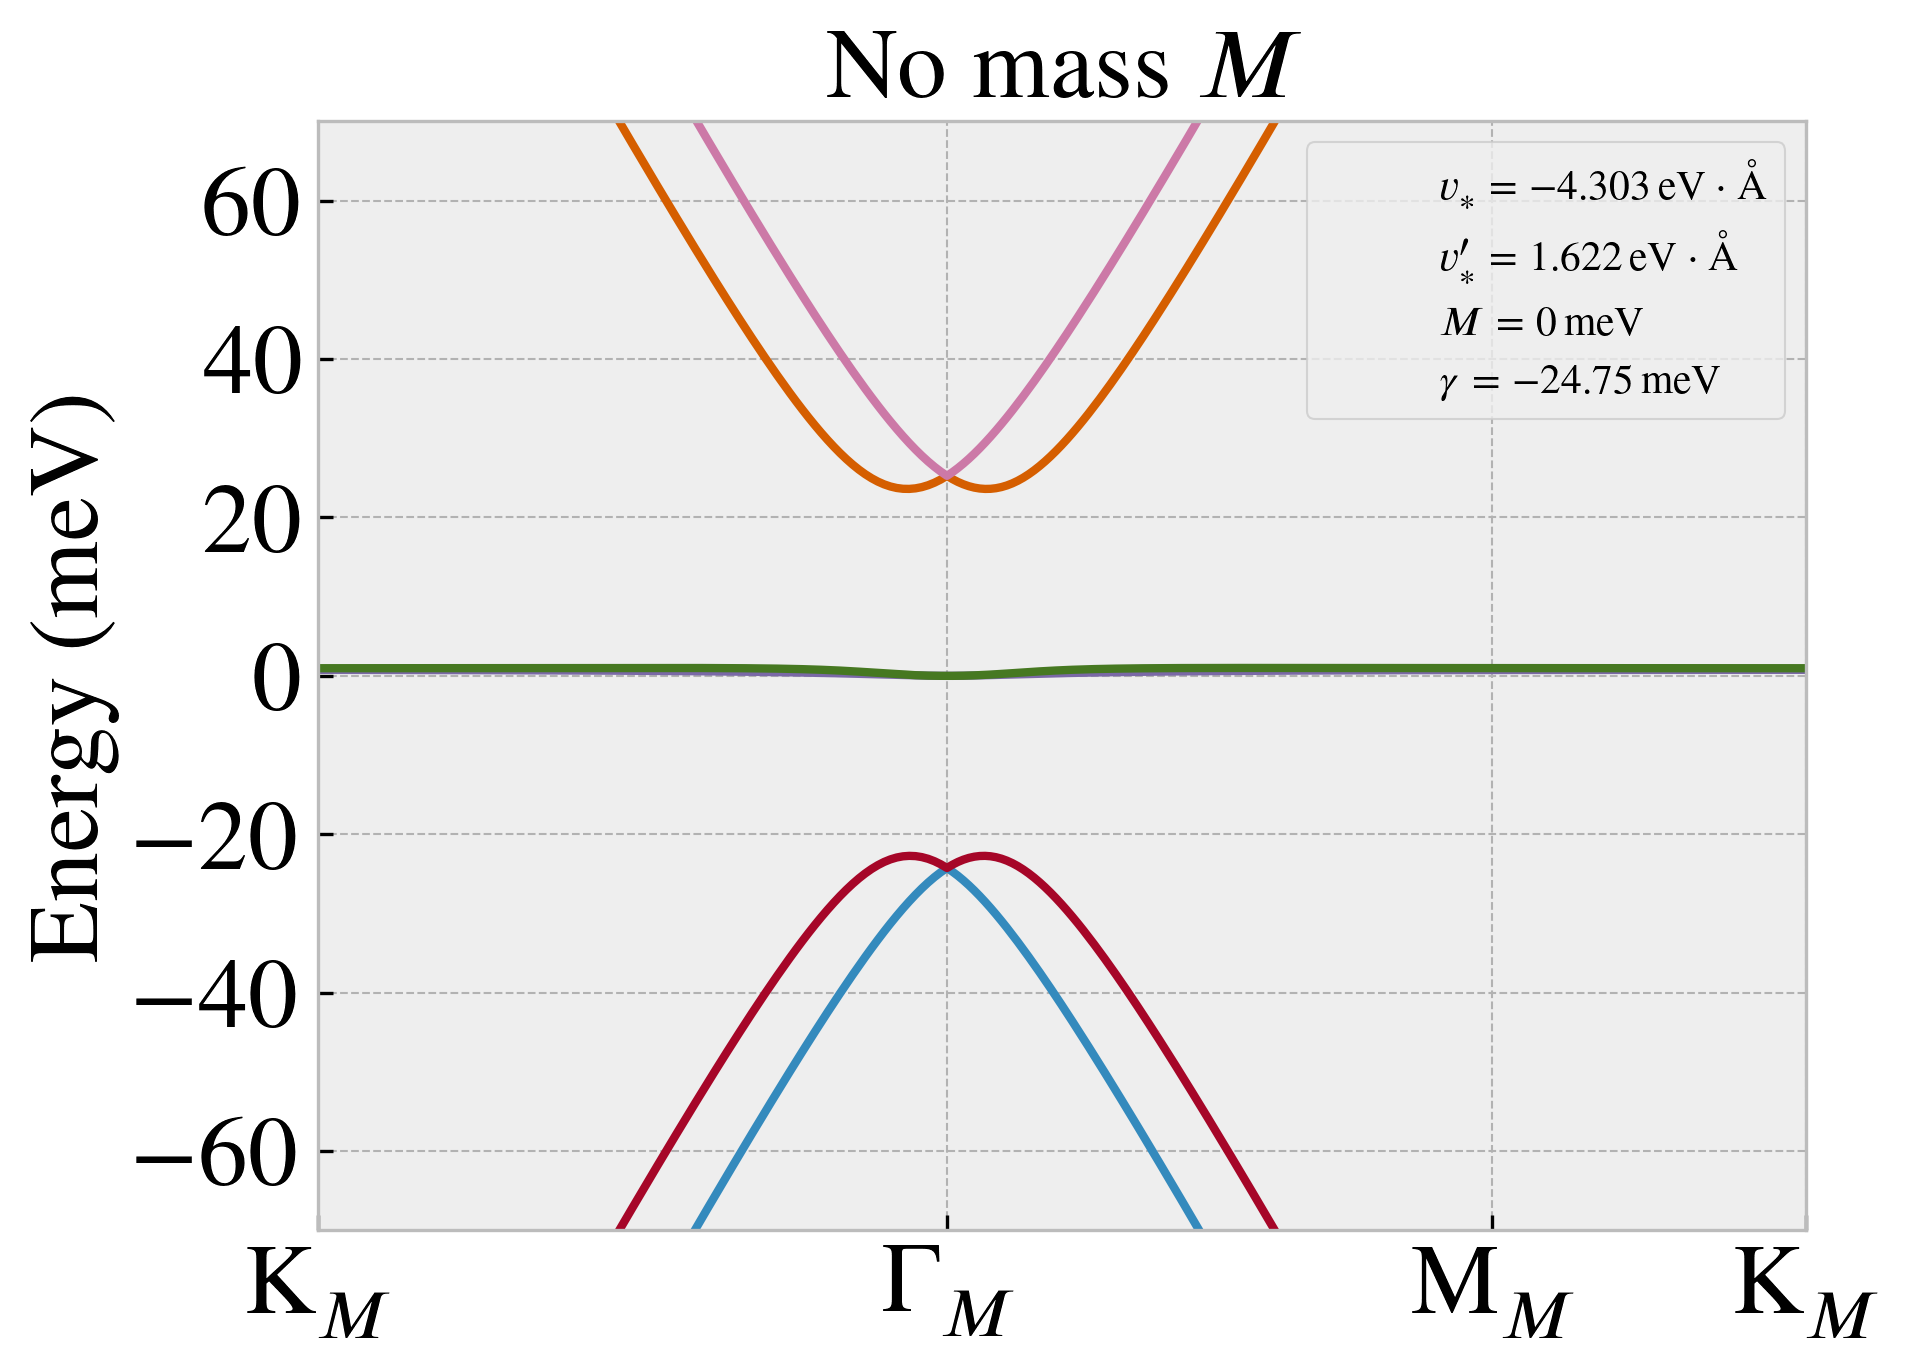
\includegraphics[height=0.35\linewidth]{fig/thf-no_M.png} \hfill
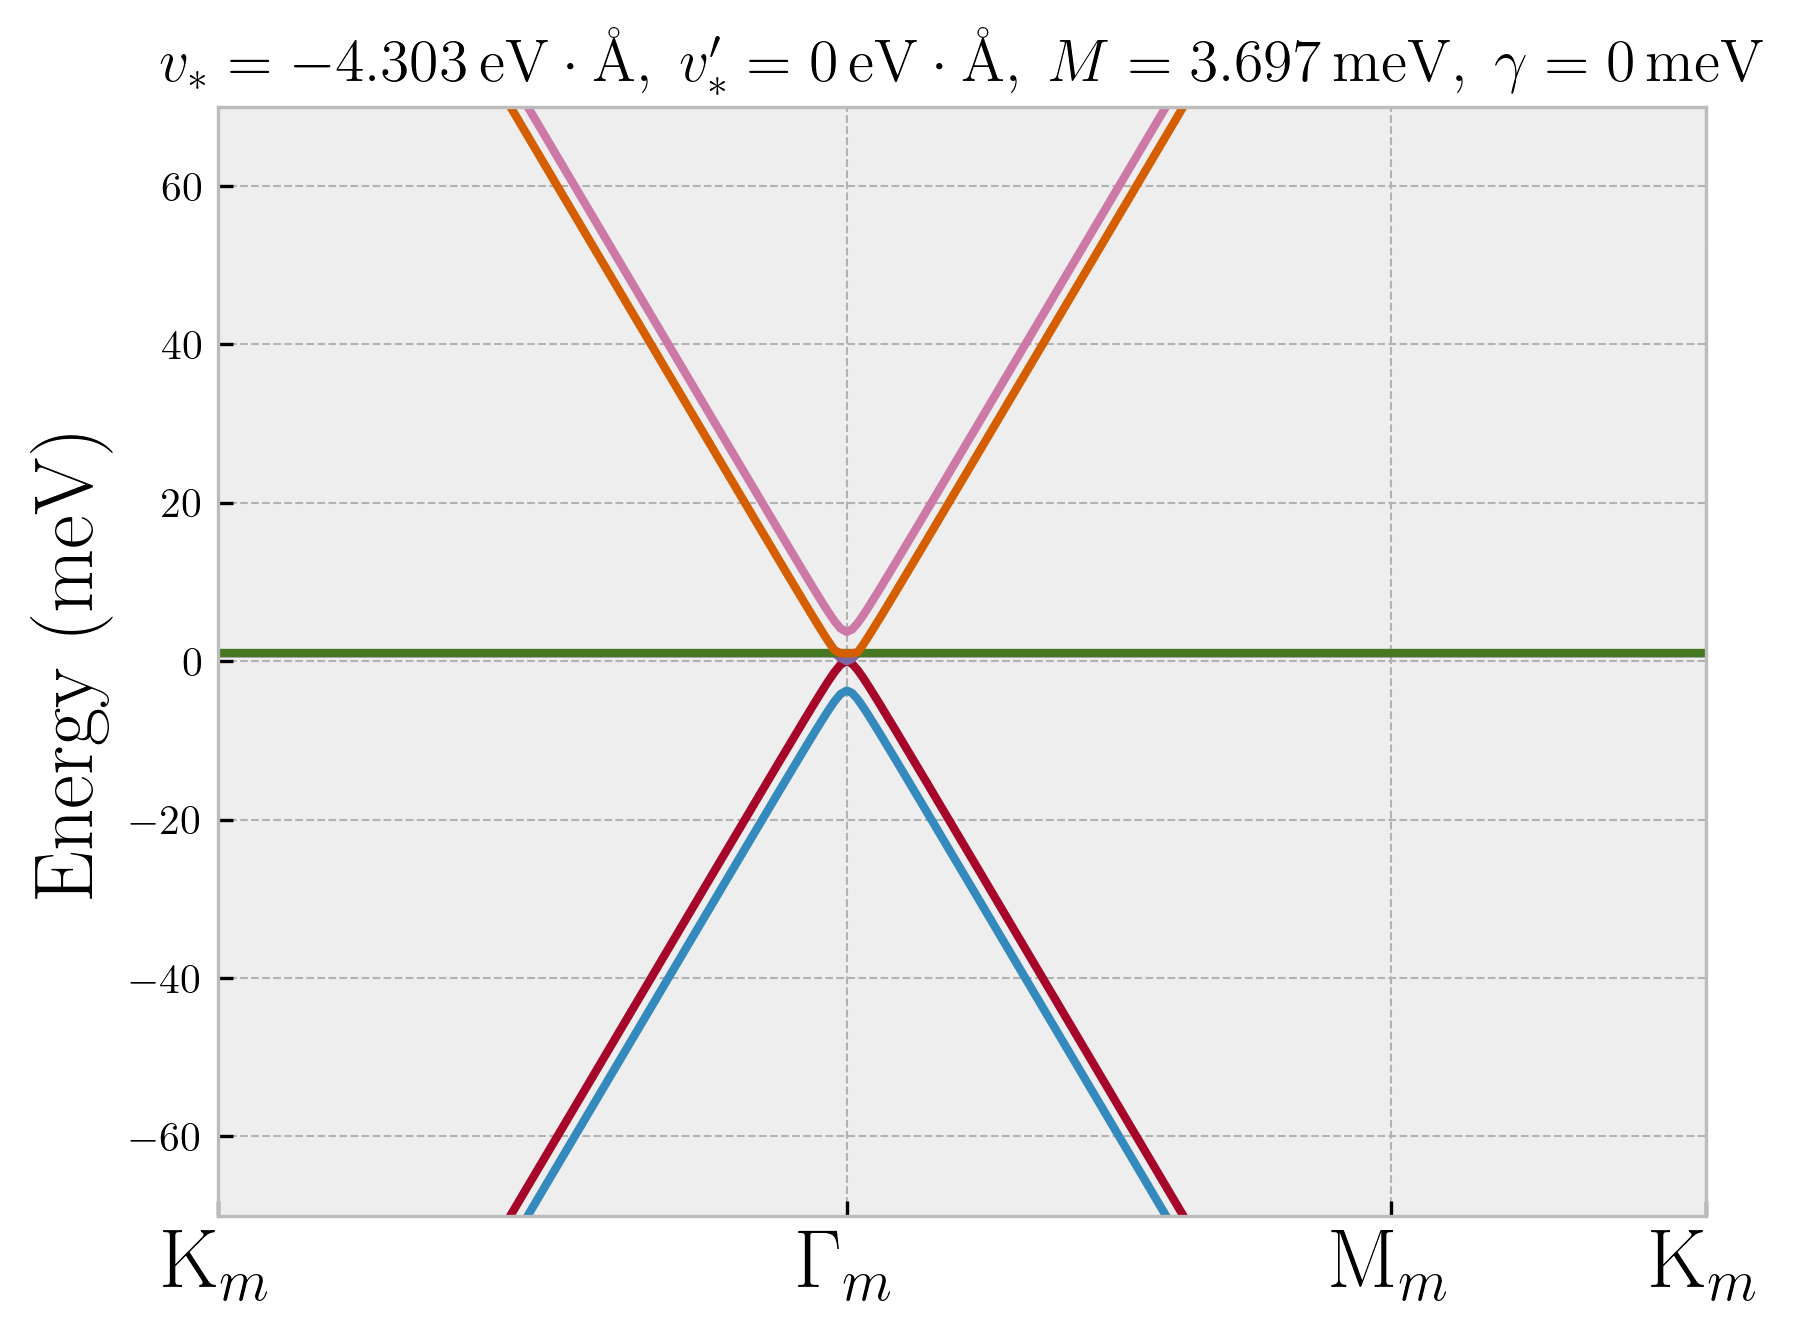
\includegraphics[height=0.35\linewidth]{fig/thf-no_coupling.png}
%%%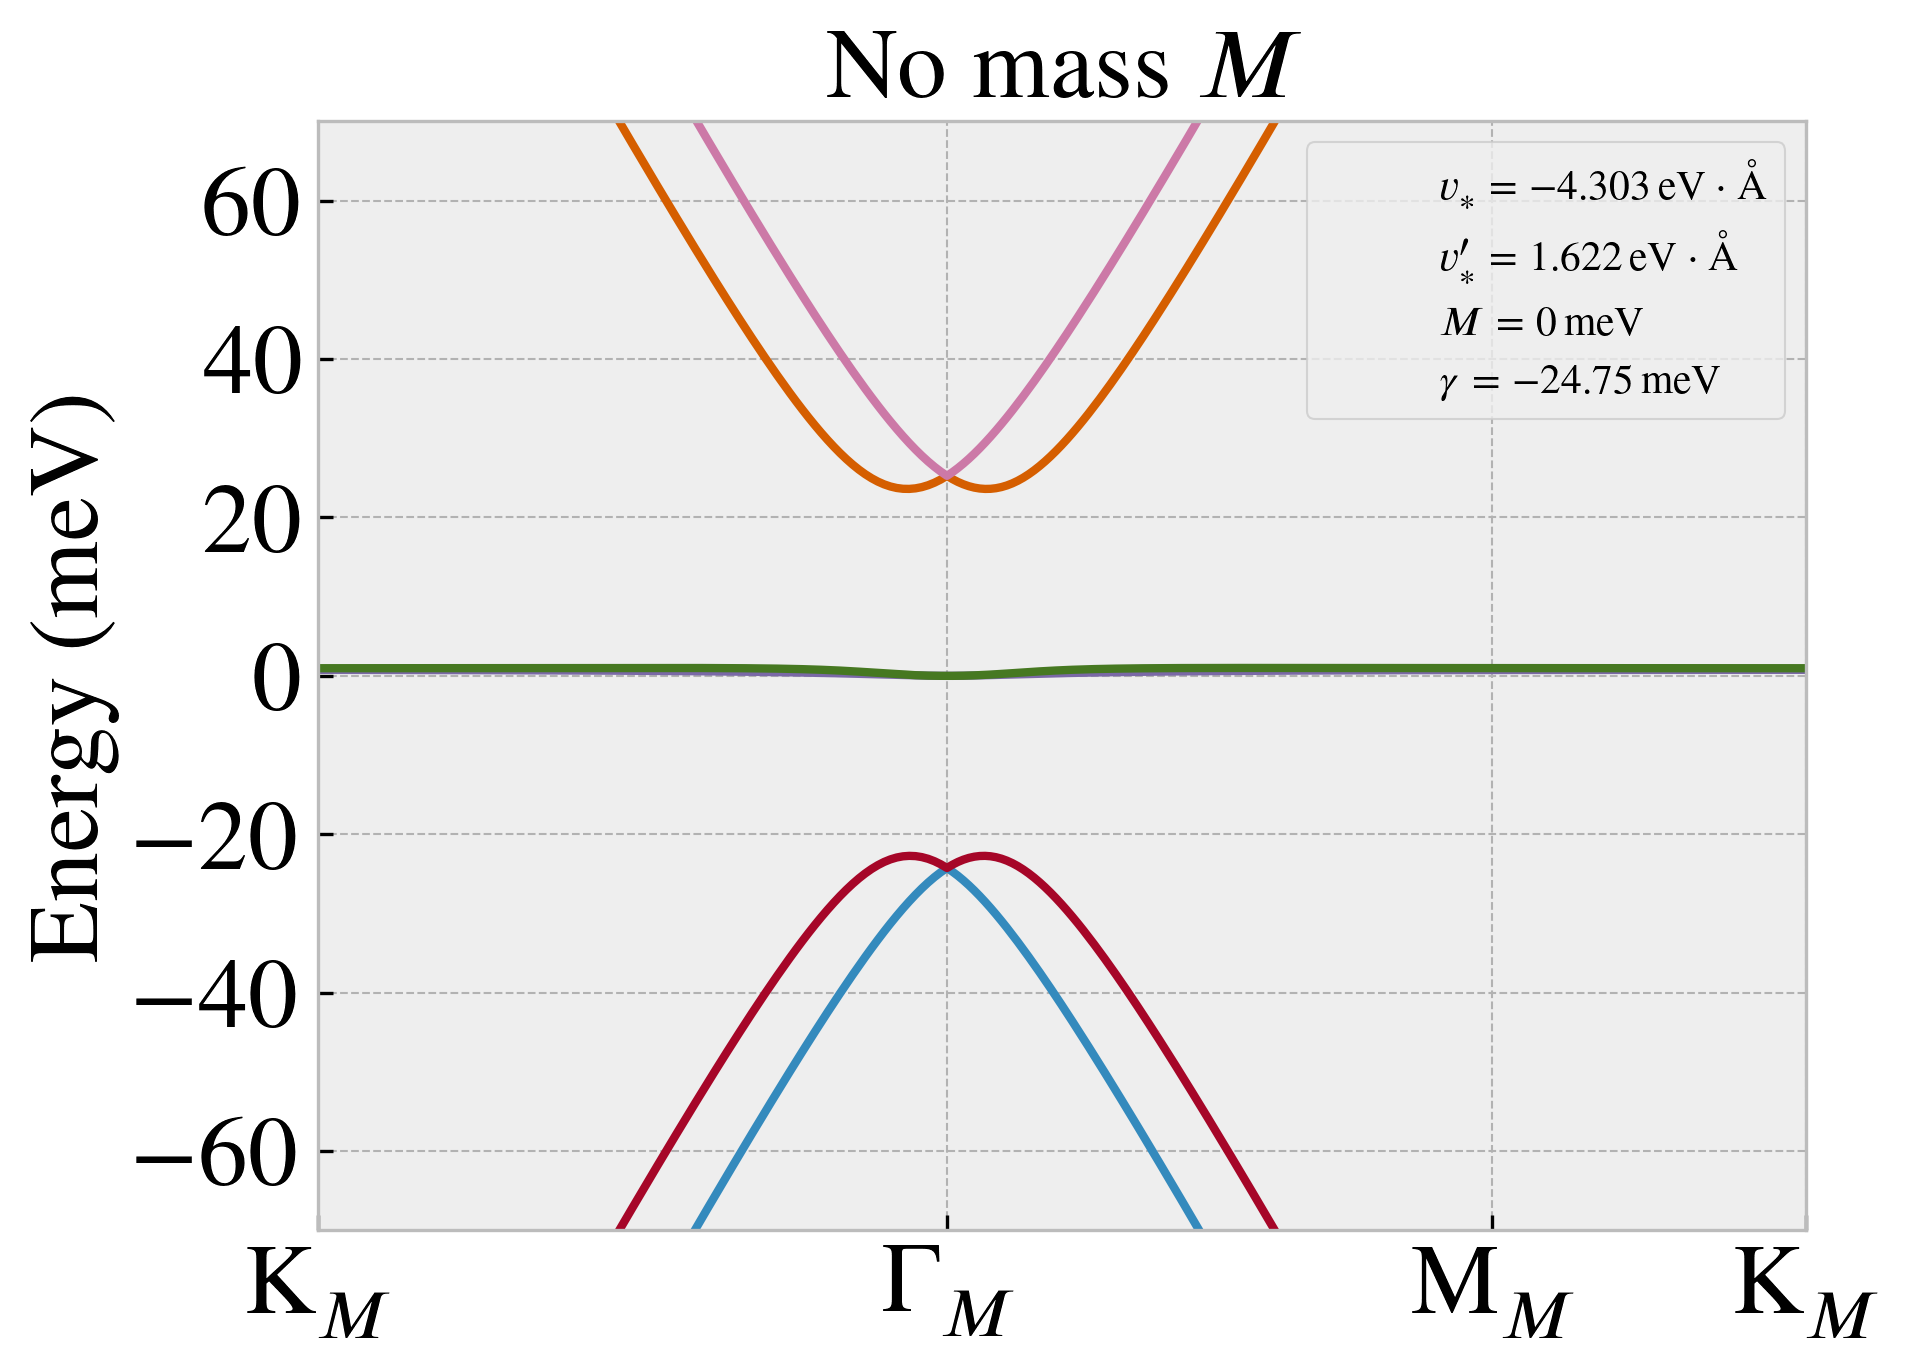
\includegraphics[height=0.35\linewidth]{fig/thf-no_M.png}
%%%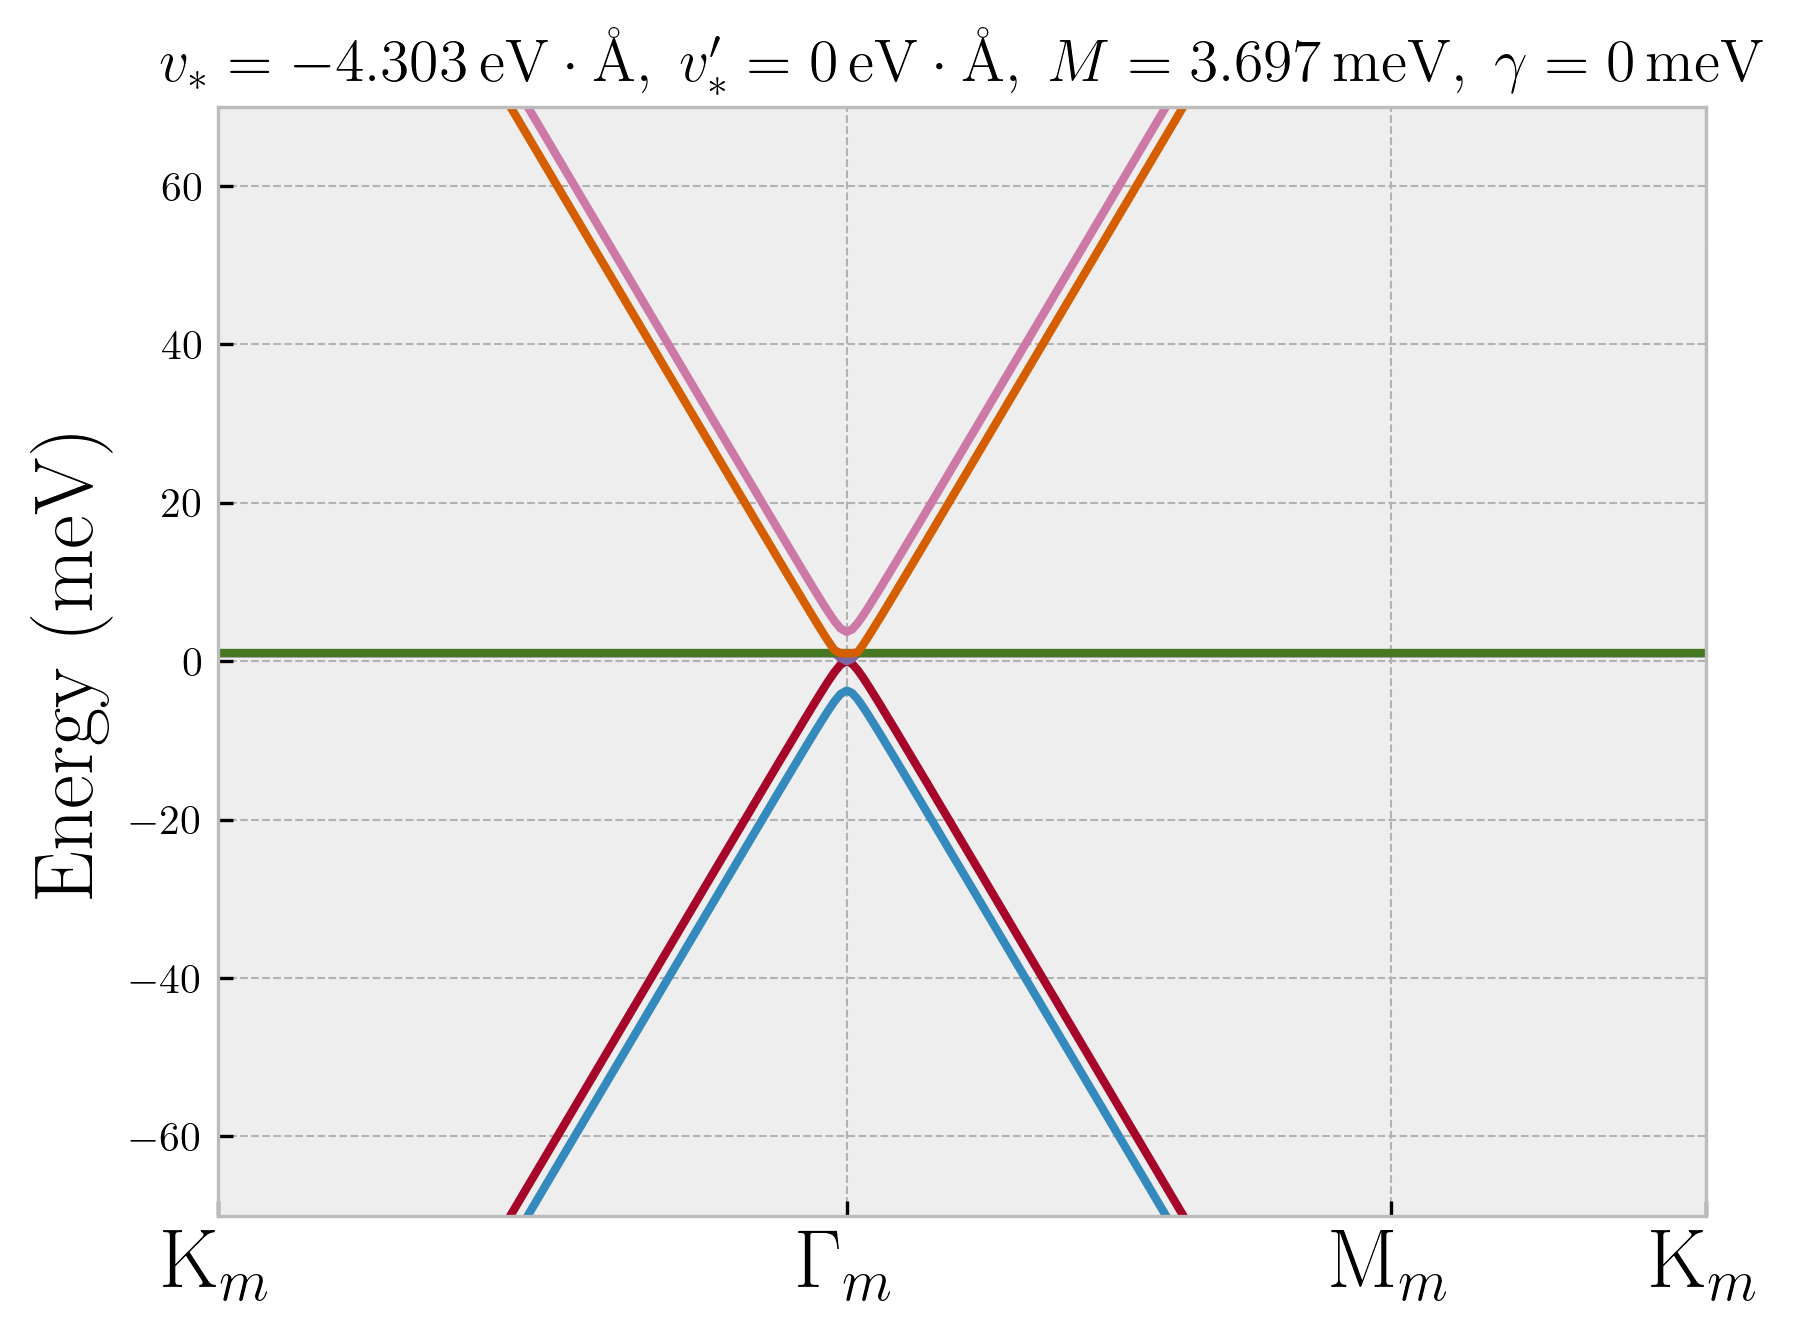
\includegraphics[height=0.35\linewidth]{fig/thf-no_coupling.png}
\caption{Band structures for the 6-band non-interacting Topological Heavy Fermion model, showing the effect of different parameters on the electronic states. Each panel illustrates a variation of the model with certain parameters set to zero.}
\label{fig:thf-exploration}
\end{figure}

\begin{figure}[H]
\centering
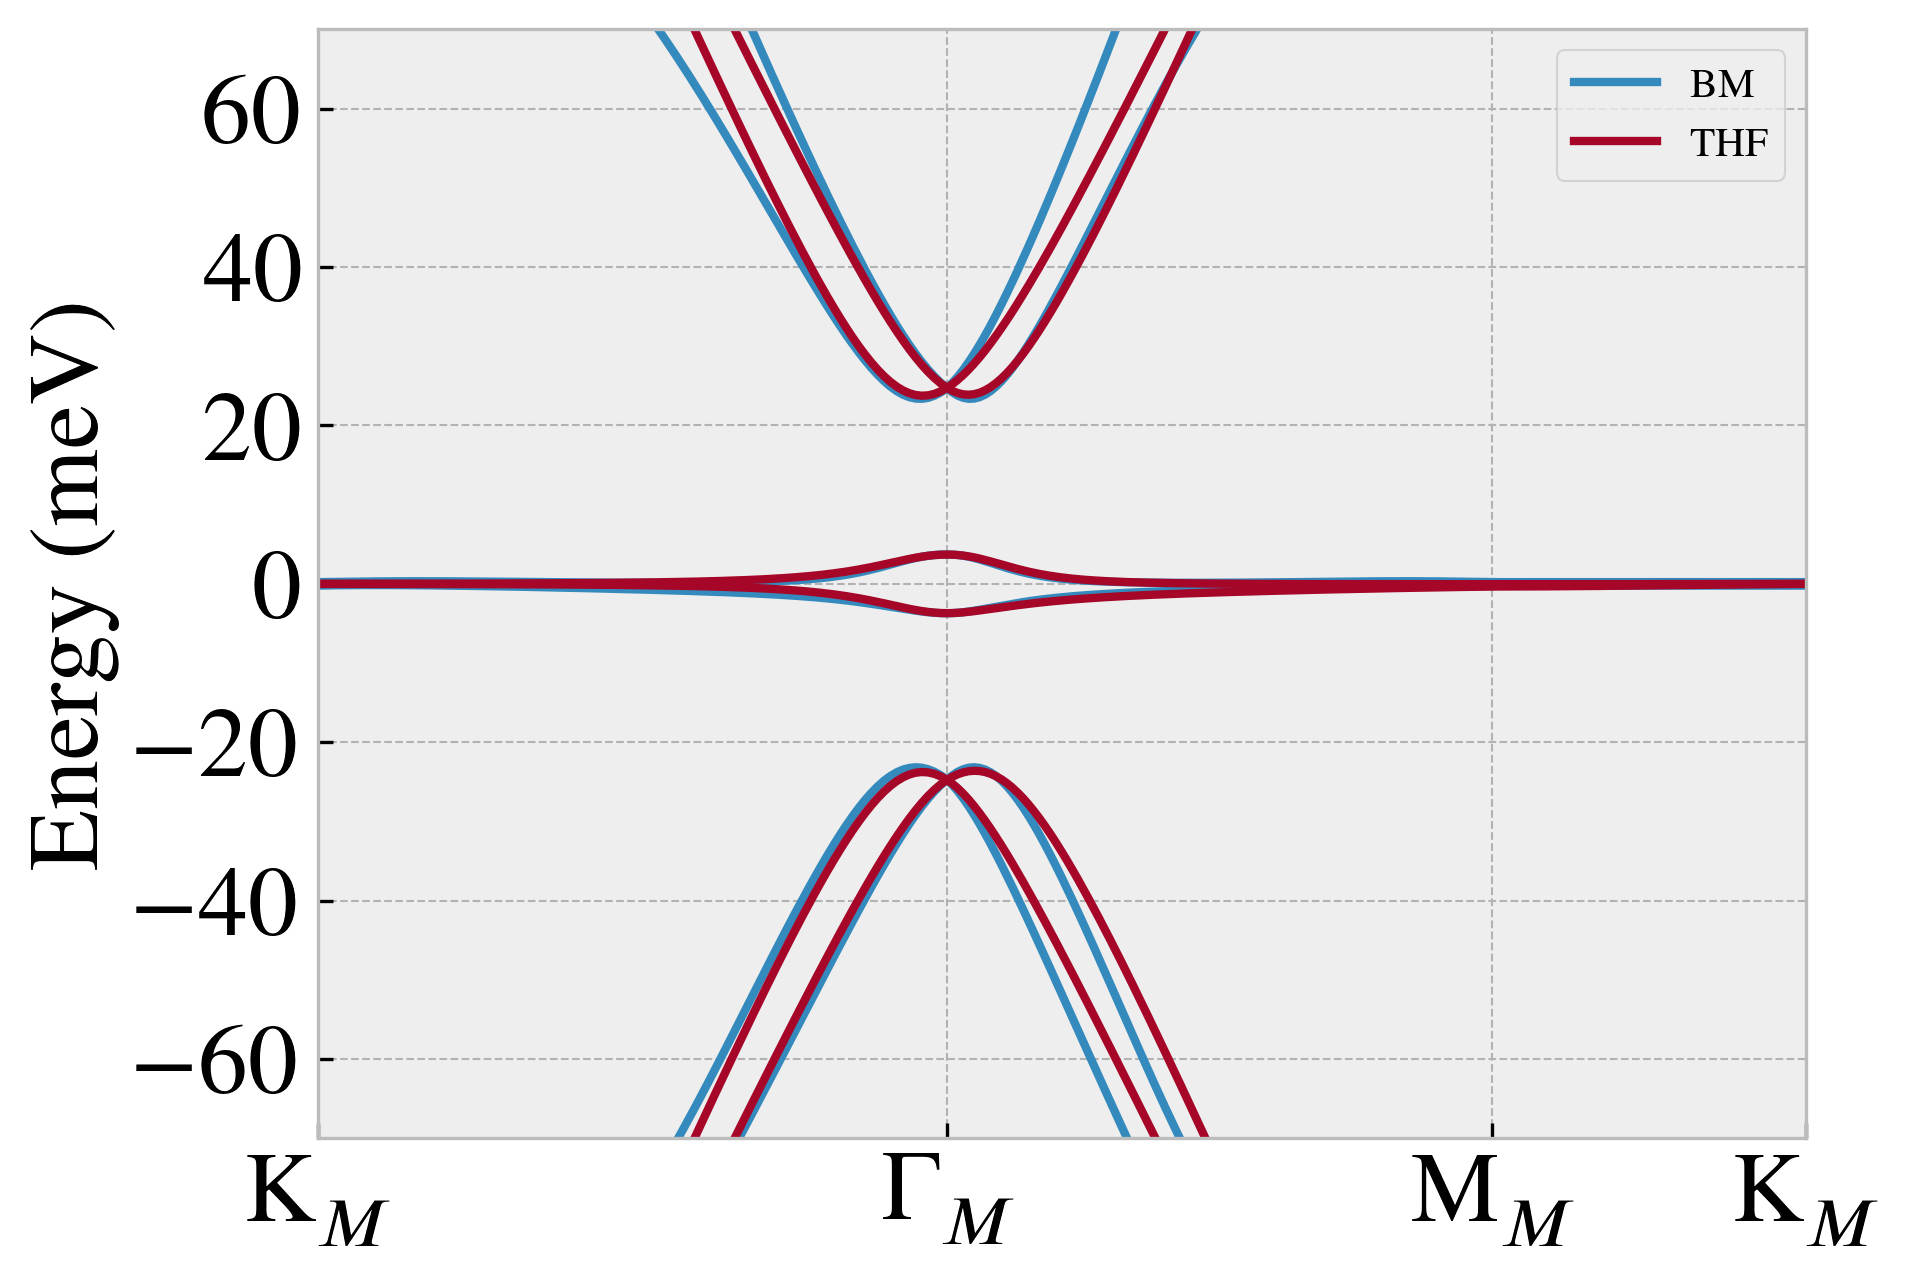
\includegraphics[width=0.9\linewidth]{fig/thf_continuum_model_vF_1.3_factor_N1.png}
\caption{THF vs BM.}
\label{fig:THF_vs_BM}
\end{figure}





%%%%%%%%%%%%%%%%%%%%%%%%%%%%%%%%%%%%%%%%%%%%%%%%%%%%%%%%%%%%%%%%%%%%%%%%%%%%%%%%%%%%%%%%%%%%%%%%%%
%%%%%%%%%%%%%%%%%%%%%%%%%%%%%%%%%%%%%%%%%%%%%%%%%%%%%%%%%%%%%%%%%%%%%%%%%%%%%%%%%%%%%%%%%%%%%%%%%%


%%%%%%%%%%%%%%%%%%%%%%%%%%%%%%% COMMENT THIS TO COMPILE main.tex %%%%%%%%%%%%%%%%%%%%%%%%%%%%%%%%
%%-----
%% Referências bibliográficas
%%-----
\addcontentsline{toc}{chapter}{\bibname}
%\bibliographystyle{abntex2-num}
\bibliography{citations}
\bibliographystyle{ieeetr}
\end{document}
%%%%%%%%%%%%%%%%%%%%%%%%%%%%%%% COMMENT THIS TO COMPILE main.tex %%%%%%%%%%%%%%%%%%%%%%%%%%%%%%%%
